\documentclass[10pt,a4paper,english,italian]{article}
\usepackage[T1]{fontenc}
\usepackage[latin1]{inputenc}
\usepackage{babel}
\usepackage{color}
\usepackage{amssymb}
\usepackage{amsmath}
\usepackage{epsfig}
\usepackage{tabularx}
\usepackage{multirow}
\usepackage{subfigure}
\usepackage{babel}
\usepackage{verbatim}
\usepackage{fancyhdr}
\usepackage{psfrag}
\usepackage{listings}
\usepackage{../common/espacs}

\setlength{\textwidth}{100ex}
\setlength{\oddsidemargin}{0ex}

\pagestyle{fancy}
\headheight 35pt

\rhead{\copyright~Copyright 2006 T. Passerini}

\makeatother

\title{Esercitazione 2\\
Addenda}
\author{T. Passerini}

\begin{document}
\lstset{language=[ISO]C++}
\maketitle 

A partire dalla soluzione dell'esercitazione 2

\begin{enumerate}

\item modificare il codice sorgente in modo da ottenere un grafico che
illustri le propriet\`a di convergenza del metodo risolutivo
implementato. Si scriva una procedura per il calcolo della soluzione
del sistema lineare, invocata dal programma \cpp{main}.

\item si faccia uso degli algoritmi generici forniti dalla libreria
STL per calcolare la norma 2 dell'errore commesso a ciascuna
iterazione dal metodo.

\end{enumerate}

\newpage
\section*{Soluzione}

\subsection*{Punto 1}

Per calcolare la soluzione del problema in
corrispondenza di differenti scelte di \cpp{M} (e quindi del passo di
discretizzazione \cpp{h}) \`e possibile
 inserire nella funzione \cpp{main} un ciclo \cpp{for} che abbia
 come variabile di controllo il numero di intervalli. All'interno del ciclo viene
 calcolato l'errore in norma infinito commesso nell'approssimare la
 soluzione esatta con quella approssimata \cpp{uh} e il risultato
 viene stampato su file.

\lstset{basicstyle=\scriptsize\sf}
\lstinputlisting[linerange={44-122},caption=Estratto dal file
fin.convergence.cpp]{./es/fin.convergence.cpp}
\lstset{basicstyle=\sf}

Il file viene aperto una volta per tutte all'esterno del ciclo. Si
noti che il costruttore della variabile \cpp{ofstream f} pu\`o
ricevere come secondo argomento un parametro che indica la modalit\`a
di gestione del file. Il comportamento di \emph{default} corrisponde alla modalit\`a
\cpp{fstream::in}, che svuota il file prima di iniziare a scrivere.

\lstset{basicstyle=\scriptsize\sf}
\begin{lstlisting}
ofstream f("fin.convergence.xy", fstream::app);
// Equivale a:
/*
   ofstream f;
   f.open("fin.convergence.xy", fstream::app);
*/
\end{lstlisting}
\lstset{basicstyle=\sf}

Il parametro \cpp{fstream::app} indica che il metodo \cpp{open}
deve aprire il file in modalit\`a \emph{append}, cio\`e in modo che i
nuovi dati siano sempre scritti in coda. Questo in particolare implica
che, se il file \`e gi\`a esistente sul filesystem, ogni invocazione
del programma causer\`a l'aggiunta dei nuovi risultati in coda a
quelli eventualmente gi\`a presenti.

Le operazioni eseguite per il calcolo della soluzione approssimata
\cpp{uh} possono essere raggruppate in una procedura, definita
all'esterno di \cpp{main}. Nella versione riportata nel \emph{Listing}
\ref{list:conv.fun}, il passaggio di parametri alla
funzione avviene \emph{per referenza}. Questo consente di aggiornare
la variabile globale \cpp{uh} durante l'esecuzione della procedura,
e quindi di calcolare correttamente la norma infinito dell'errore di
approssimazione nella funzione \cpp{main}. Si noti che
l'implementazione della funzione \cpp{solve\_GS} non cambia rispetto
al caso in cui tutti i parametri siano passati per valore: la
referenza funge da \emph{alias} per la variabile referenziata.

\lstset{basicstyle=\scriptsize\sf}
\lstinputlisting[linerange={44-53, 93-141},caption=Estratto dal file
fin.convergence.function.cpp,label=list:conv.fun]{./es/fin.convergence.function.cpp}
\lstset{basicstyle=\sf}

Lo stesso effetto del passaggio per referenza si pu\`o ottenere
passando come argomento alla funzione l'indirizzo di \cpp{uh}. In
questo caso il parametro formale di \cpp{solve\_GS} \`e un puntatore
a \emph{double}, e la sintassi all'interno della procedura va cambiata
di conseguenza.

\lstset{basicstyle=\scriptsize\sf}
\lstinputlisting[linerange={43-100,119-123,146-147},caption=Estratto dal file
fin.convergence.function.ptr.cpp,label=list:conv.fun.ptr]{./es/fin.convergence.function.ptr.cpp}
\lstset{basicstyle=\sf}

Il vettore \cpp{uh} pu\`o anche essere allocato dinamicamente: in
questo modo il ciclo di vita della variabile \`e stabilito dal
programmatore. Questo pu\`o essere utile, in generale, quando
l'allocazione di memoria \`e sottoposta ad una condizione:

\lstset{basicstyle=\scriptsize\sf}
\begin{lstlisting}
double * global_pointer = 0;
if( test )
{
  double * pointer = new double;
  ...
  global_pointer = pointer;
}
\end{lstlisting}
\lstset{basicstyle=\sf}

ma tuttavia si desidera che l'area di memoria sia accessibile anche
all'esterno dello scope locale (cio\`e non sia deallocata
automaticamente al termine dell'esecuzione del blocco \cpp{if}).

L'allocazione dinamica di \cpp{uh} richiede l'utilizzo appropriato
di istruzioni \cpp{delete} per evitare \emph{memory leak}.

\lstset{basicstyle=\scriptsize\sf}
\lstinputlisting[linerange={99-148},caption=Estratto dal file
fin.convergence.function.alloc.cpp, 
label=list:conv.fun.alloc]{./es/fin.convergence.function.alloc.cpp}
\lstset{basicstyle=\sf}

D'altra parte la gestione dell'allocazione tramite
puntatori non garantisce dalla perdita di memoria nel caso di
fallimento del programma: se l'esecuzione abortisce, vengono
deallocate le variabili dalla pila (\emph{stack}) del programma (e tra queste i puntatori
istanziati) ma non viene automaticamente liberata la
memoria allocata dinamicamente (nello \emph{heap}).

\`E possibile forzare la deallocazione delle variabili residenti nello
\emph{heap} ricorrendo alla gestione delle eccezioni (di cui si
parler\`a pi\`u avanti nel corso). Un'alternativa pi\`u pratica \`e
ricorrere all'\emph{auto pointer} reso disponibile dalla STL.

\lstset{basicstyle=\scriptsize\sf}
\lstinputlisting[linerange={13-13, 44-54, 100-101, 112-114,147-148},
caption=Estratto dal file
fin.convergence.function.alloc.smart.cpp,
label=list:conv.fun.alloc.smart]{./es/fin.convergence.function.alloc.smart.cpp}
\lstset{basicstyle=\sf}

Il puntatore \emph{auto}, oltre ad allocare un oggetto,
lo ``possiede''. In questo modo \`e possibile fare in modo che la
memoria puntata sia deallocata nel momento in cui il puntatore viene deallocato.

Il concetto di ``possesso'' richiede un trattamento particolare per
gli \emph{auto pointers}, quando questi siano utilizzati come
parametri di funzione. Per trasferire alla funzione il puntatore alla
variabile allocata, ma \emph{non} il possesso della variabile stessa,
\`e necessario che il parametro sia una riferimento costante ad un
\emph{auto pointer}. Se il possesso fosse trasferito alla funzione,
al termine dell'esecuzione stessa la variabile puntata sarebbe
deallocata (si veda \cite{Josuttis}).

Dopo l'esecuzione del programma, il file \texttt{fin.convergence.xy}
contiene un elenco di coppie ascissa-ordinata che possono essere
rappresentate in un grafico. A questo scopo si pu\`o ricorrere a
\texttt{Gnuplot}, software per la visualizzazione di dati che viene
controllato da linea di comando o tramite \emph{script}.

\lstset{basicstyle=\scriptsize\sf}
\lstinputlisting[caption=File \texttt{plot.convergence.gnu}: script
\texttt{Gnuplot} per la visualizzazione dei
risultati.]{./es/plot.convergence.gnu}
\lstset{basicstyle=\sf}

L'istruzione \texttt{set term} assegna le propriet\`a del terminale
grafico; per la visualizzazione delle propriet\`a di convergenza del
metodo di Gauss-Seidel \`e stata impostata la scala logaritmica su
entrambi gli assi, con i comandi \texttt{set logscale}, ed \`e stata
attivata la visualizzazione del reticolo (\texttt{set grid}). La
legenda viene attivata e posizionata con il comando \texttt{set
  key}. Il comando di visualizzazione \`e \texttt{plot} (abbreviato in
\texttt{p}), che riceve come parametro il file in ingresso seguito
dalle opzioni \texttt{using} (\texttt{u}, per scegliere quali colonne
utilizzare come sorgenti di dati), \texttt{with} (\texttt{w}, per
scegliere lo stile di visualizzazione: \texttt{lp} sta per
\texttt{linepoint}), \texttt{tag} (\texttt{t}, \`e l'etichetta da
associare alla linea nella legenda). Il grafico viene salvato su file
(\texttt{set output}), in formato Postscript. Per ulteriori
informazioni si rimanda alla documentazione di Gnuplot
(\texttt{http://www.gnuplot.info/} oppure \texttt{man gnuplot}).
%
\begin{figure}
\begin{center}
\psfrag{linf}{$\norm{ e }_{\hilbertL{\infty}{\Omega}}$}
\includegraphics[height=0.45\textwidth,angle=-90]{./figures/eps/fin.convergence.eps}
\caption{Risultati sperimentali di convergenza per il problema termico
dell'aletta.}
\label{fig:fin:conv}
\end{center}
\end{figure}

\subsection*{Punto 2}

Per valutare l'errore commesso ad ogni iterazione del metodo di
Gauss-Seidel, pu\`o essere esplicitamente istanziato il vettore
contenente l'incremento tra due iterate successive, in modo da
memorizzarne il valore relativo a ciascun nodo: a questo punto il calcolo
dell'errore richiede delle operazioni vettoriali, che implicano la
scansione elemento per elemento. La STL mette a disposizione degli
\emph{algoritmi generici} che consentono di rendere pi\`u pratica ed
efficiente la manipolazione dei contenitori, ad esempio la ricerca, la
copia o l'ordinamento di valori. Per i contenitori sequenziali di tipi
numerici \`e disponibile la libreria \emph{numeric}, che implementa
tra gli altri un algoritmo di sommazione elemento per elemento
(\cpp{accumulate()}) e un algoritmo di prodotto interno tra due
sequenze (\cpp{inner\_product()}).

Il calcolo dell'errore pu\`o essere ottenuto ad esempio nel modo
seguente
\lstset{basicstyle=\scriptsize\sf}
\lstinputlisting[linerange={66-99},
caption=Estratto dal file
fin.inner.cpp,
label=list:inner]{./es/fin.inner.cpp}
\lstset{basicstyle=\sf}

In questo modo la norma euclidea di \cpp{epsilon} \`e
calcolata come prodotto interno del vettore per se stesso. In
alternativa \`e possibile utilizzare la procedura \cpp{accumulate}:
in tal caso \cpp{epsilon} contiene i quadrati della differenza tra
due iterate successive, valutata in ciascun nodo.
\lstset{basicstyle=\scriptsize\sf}
\lstinputlisting[linerange={66-100},
caption=Estratto dal file
fin.accumulate.cpp,
label=list:accumulate]{./es/fin.accumulate.cpp}
\lstset{basicstyle=\sf}

Si noti che, in entrambi i casi, occorre fornire agli algoritmi un
valore iniziale (l'ultimo parametro nella chiamata delle
funzioni). Per approfondimenti si faccia riferimento a \cite{Josuttis}.


\bibliographystyle{siam}
\bibliography{../common/bibliography}

\end{document}
